\documentclass[11pt]{article}
\usepackage[utf8]{inputenc}
\usepackage[letterpaper,top=1in,right=1in,left=1in,bottom=1in]{geometry}
%-------------------Packages Required-----------------------------------------%

\usepackage{amsmath}
%\usepackage[top=25.4truemm,bottom=25.4truemm,left=25.4truemm,right=25.4truemm]{geometry}
\usepackage{mathrsfs}
\usepackage{amsfonts}
\usepackage{graphicx}
\usepackage{caption}   
\usepackage{subcaption}          
\usepackage{breqn}                      
\usepackage{booktabs}    
\usepackage{threeparttable}
\usepackage{tabularx} 
\usepackage[toc,page]{appendix}     
\usepackage{enumitem}  
\usepackage{lscape} 
\usepackage{ascmac}     
\usepackage{rotating}
\usepackage{url}
\usepackage{setspace}  
\usepackage{adjustbox}
\usepackage{stackengine}
\usepackage{pdfpages}
\usepackage{graphicx}
\usepackage{hyperref} 
\usepackage{placeins}
\usepackage{comment}
\hypersetup{colorlinks=true, citecolor=blue, urlcolor  = blue, linkcolor = blue} 
\usepackage[multiple]{footmisc} 
\graphicspath{Figure/}
\usepackage{flafter}
\usepackage{siunitx}
\usepackage{bbding}
\usepackage{makecell}

\begin{document}

\subsection{Unrestricted}
\begin{figure}[ht!]
        \centering
       \caption{Sorted Group Average Treatment Effects, estimated with Random Forest (All Grades)} 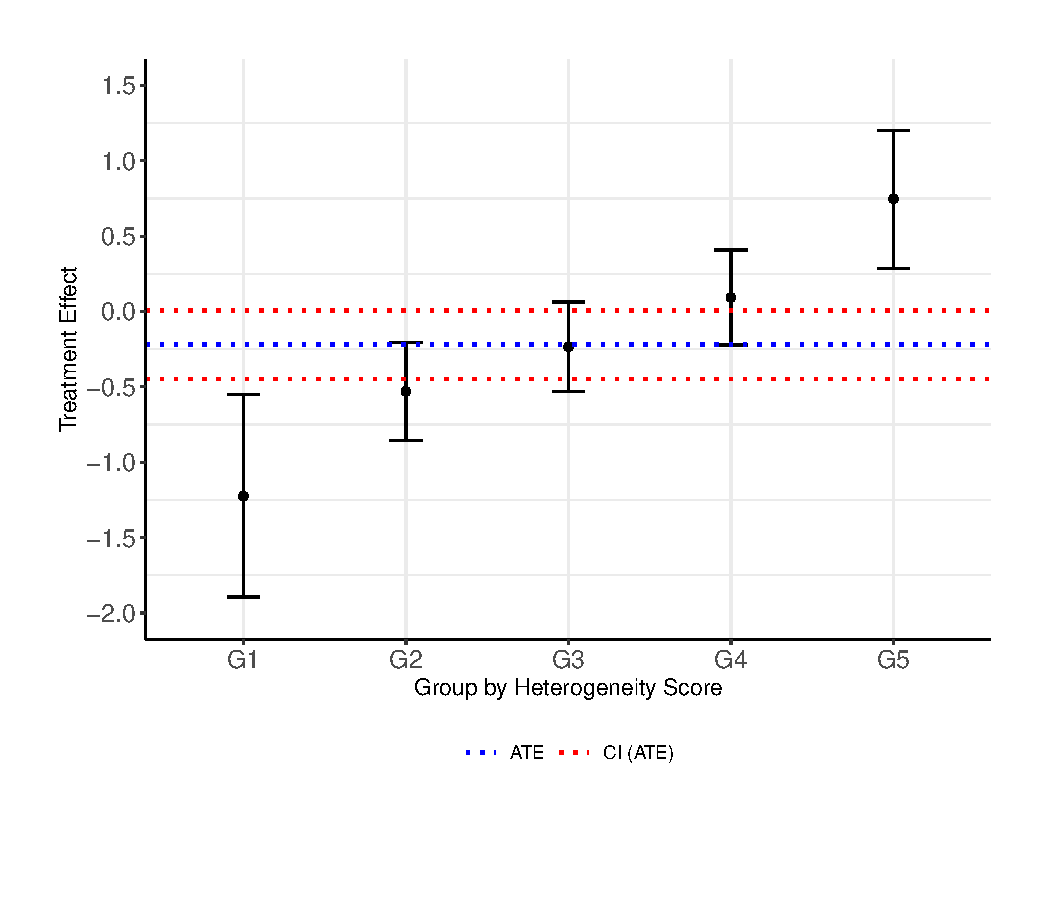
\includegraphics[width = 5in]{Replication_Liberia/heteffect_ML_All.pdf}
        \caption*{Note: Standard errors are clustered at the academy-grade group level. The covariates used in the analysis are combinations of distances from the 10th, 25th, 50th, 75th, and 90th percentile levels of instruction in grades 1 through 4, resulting in 625 covariates.}
\end{figure}

\begin{figure}[ht!]
        \centering
       \caption{Sorted Group Average Treatment Effects, estimated with Random Forest (Grades 1 \& 2)} 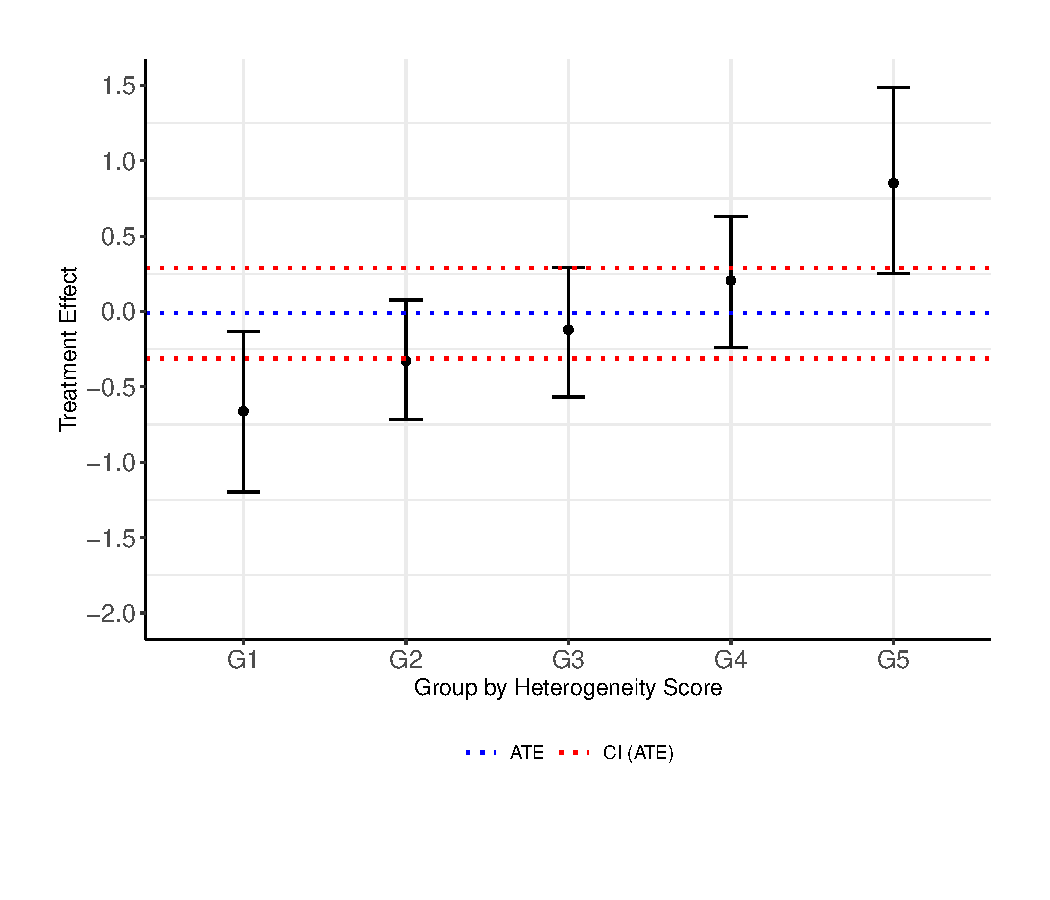
\includegraphics[width = 5in]{Replication_Liberia/heteffect_ML_Grade1_2.pdf}
        \caption*{Note: Standard errors are clustered at the academy-grade group level. The covariates used in the analysis are combinations of distances from the 10th, 25th, 50th, 75th, and 90th percentile levels of instruction in grades 1 and 2, resulting in 25 covariates.}
\end{figure}


\begin{figure}[ht!]
        \centering
       \caption{Sorted Group Average Treatment Effects, estimated with Random Forest (Grades 3 \& 4)} 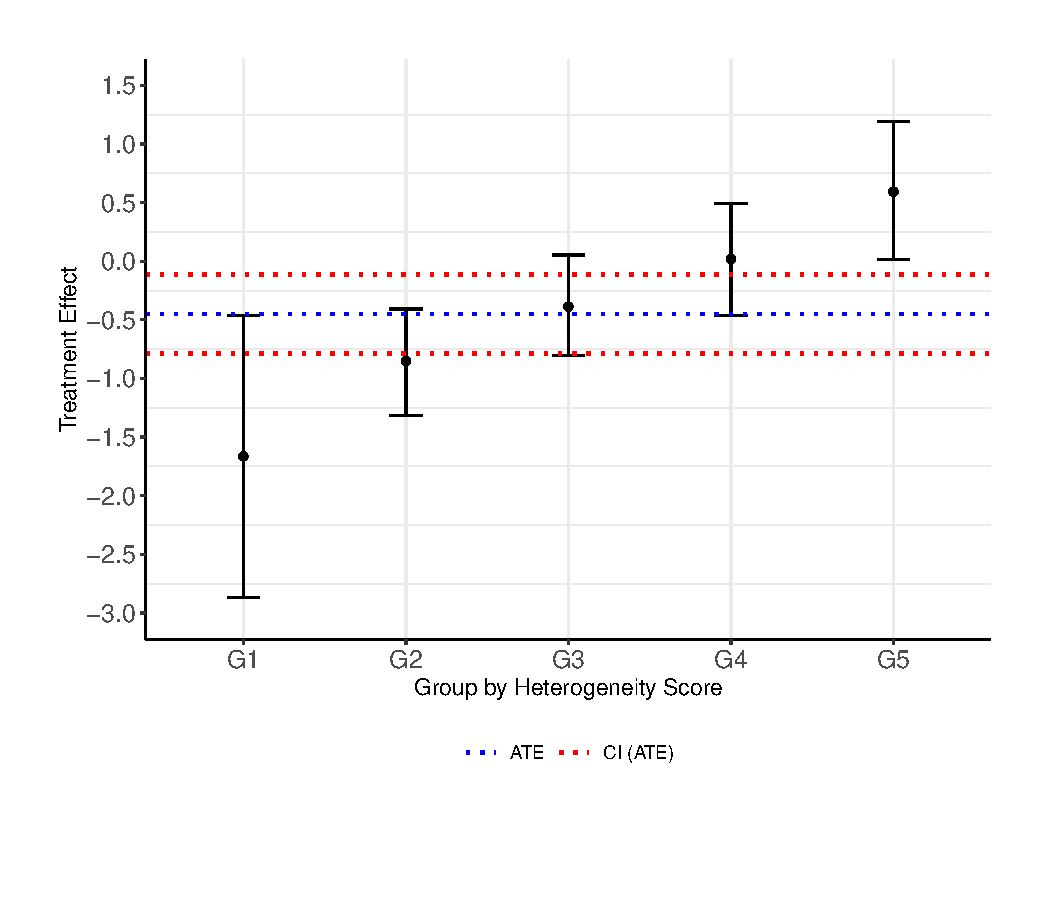
\includegraphics[width = 5in]{Replication_Liberia/heteffect_ML_Grade3_4.pdf}
        \caption*{Note: Standard errors are clustered at the academy-grade group level. The covariates used in the analysis are combinations of distances from the 10th, 25th, 50th, 75th, and 90th percentile levels of instruction in grades 3 and 4, resulting in 25 covariates.}
\end{figure}

\clearpage
\subsection{Restricted: The instructional levels for Grades 2 and 4 are limited to the 75th and 90th percentiles.}

\begin{figure}[ht!]
        \centering
       \caption{Sorted Group Average Treatment Effects, estimated with Random Forest (All Grades)} 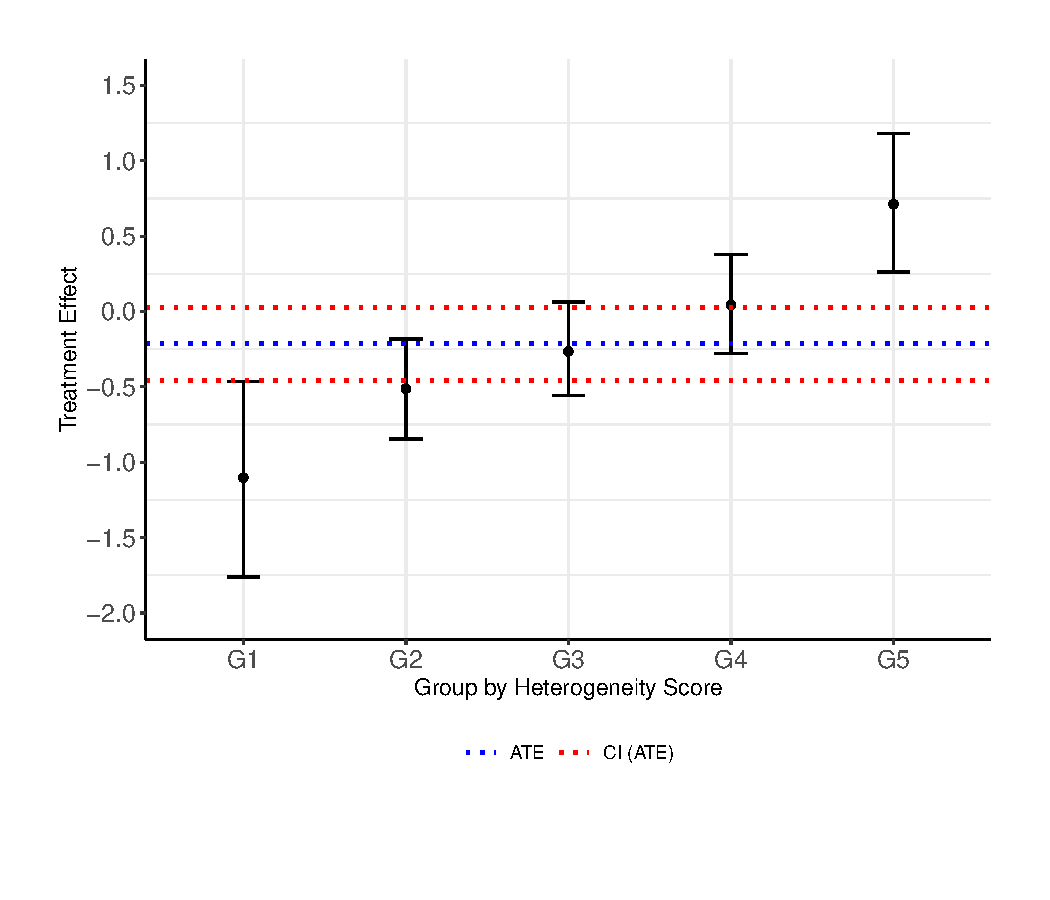
\includegraphics[width = 5in]{Replication_Liberia/heteffect_ML_All_Restricted.pdf}
        \caption*{Note: Standard errors are clustered at the academy-grade group level. The covariates used in the analysis are combinations of distances from the 10th, 25th, 50th, 75th, and 90th percentile levels of instruction in grades 1 through 4, resulting in 100 covariates.}
\end{figure}

\begin{figure}[ht!]
        \centering
       \caption{Sorted Group Average Treatment Effects, estimated with Random Forest (Grades 1 \& 2)} 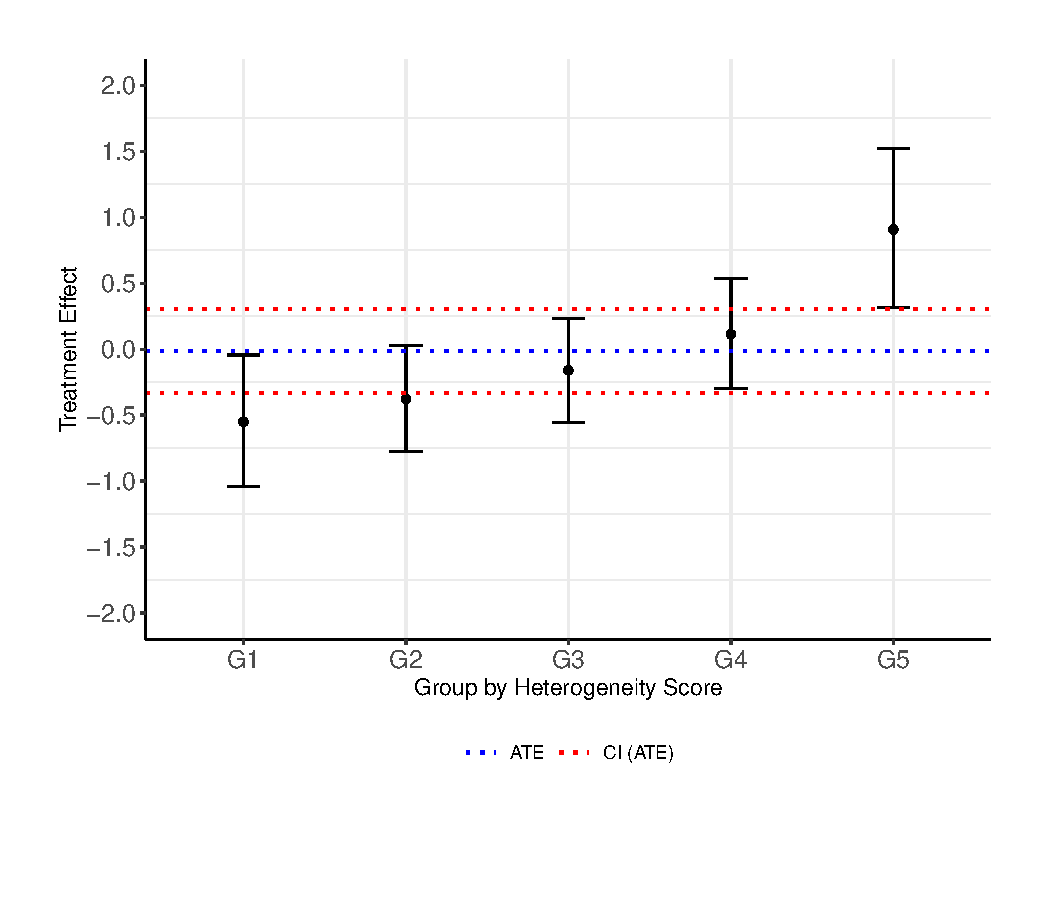
\includegraphics[width = 5in]{Replication_Liberia/heteffect_ML_Grade1_2_Restricted.pdf}
        \caption*{Note: Standard errors are clustered at the academy-grade group level. The covariates used in the analysis are combinations of distances from the 10th, 25th, 50th, 75th, and 90th percentile levels of instruction in grades 1 and 2, resulting in 10 covariates.}
\end{figure}


\begin{figure}[ht!]
        \centering
       \caption{Sorted Group Average Treatment Effects, estimated with Random Forest (Grades 3 \& 4)} 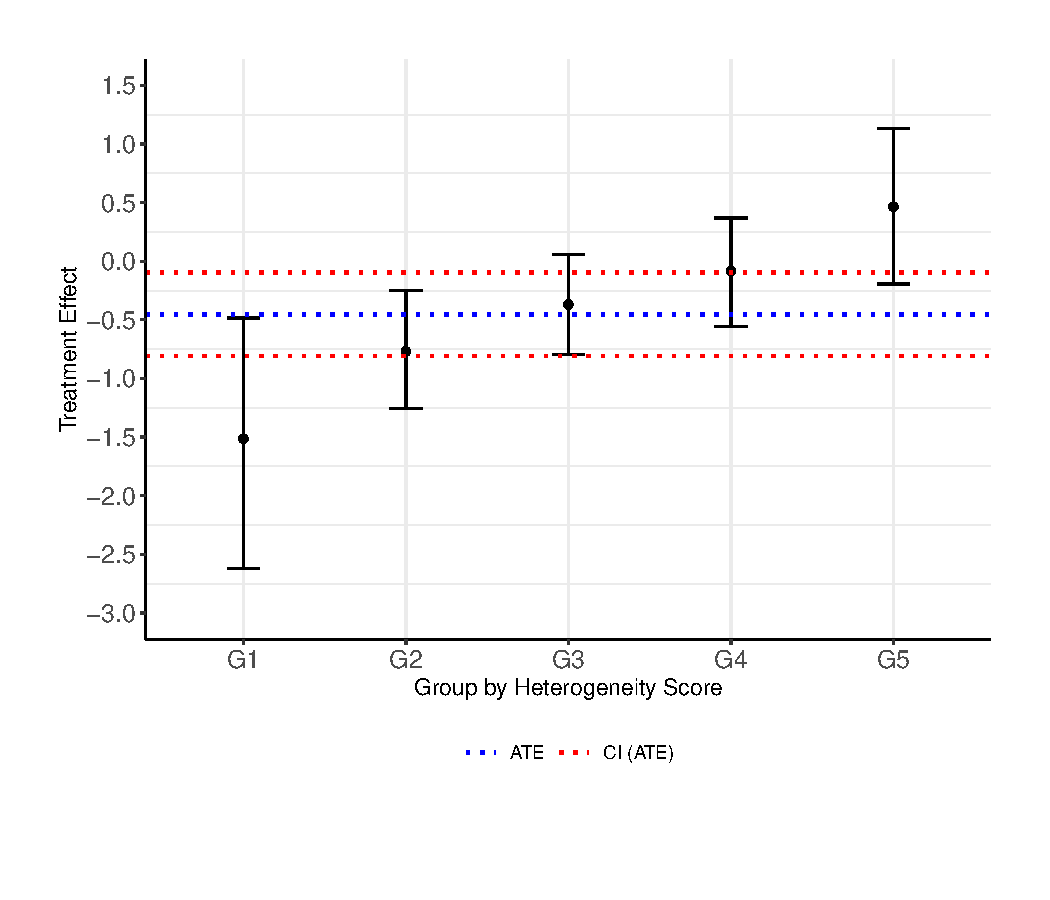
\includegraphics[width = 5in]{Replication_Liberia/heteffect_ML_Grade3_4_Restricted.pdf}
        \caption*{Note: Standard errors are clustered at the academy-grade group level. The covariates used in the analysis are combinations of distances from the 10th, 25th, 50th, 75th, and 90th percentile levels of instruction in grades 3 and 4, resulting in 10 covariates.}
\end{figure}

\end{document}